\documentclass[twoside]{article}

\usepackage{amsmath}
\usepackage{amsfonts}
\usepackage{graphicx}
\usepackage{multirow}
\usepackage{fontspec}
\usepackage{hyperref}
\usepackage{xepersian}
% Font Settings ======================
\setlatintextfont{LinLibertine}[Path = fonts/latin/]
\settextfont{HMXKayhan}[
Path = fonts/fa/ ,
BoldFont = HMXKayhanBd]
% Graphic Settings ===================
\graphicspath{{images/}}
\DeclareGraphicsExtensions{.jpeg,.png,.jpg}


\title{\Huge پیش گزارش آزمایش 4 آز مدار منطقی }
\author{\Large علی دهقانی ، ماهان بیهقی}
\date{دانشگاه صنعتی شریف}

\begin{document}
	\maketitle
	\newpage
	\section*{نام آزمایش}
	شیفت رجیسترها
	
	\section*{اهداف آزمایش}
	پیاده سازی یک شیفت رجیستر با تراشه 7495
	
	\section*{شرح آزمایش}
	
	\subsection*{لیست تراشه ها و قطعات مورد نیاز}
	\href{https://www.jameco.com/Jameco/Products/ProdDS/50770NSC.pdf}{تراشه 7495} ، مالتی پلکسر های 2 به 1
	
	\subsection*{شرح آزمایش}
	
	شکل اتصالات داخلی تراشه 7495 در شکل 1 مشخص شده است. از این تراشه میتوان برای ساخت یک شیفت رجیستر با ورودی های موازی و سریال استفاده کرد. همچنین خروجی شیفت رجیستر میتواند به صورت موازی باشد یعنی این تراشه در کل یک شیفت رجیستر PIPO به شمار میرود که قابلیت خروجی سریال را هم دارد.
	شمارنده جانسون یا یا شمارنده حلقه هم نوعی شمارنده سنکرون متشکل از n فلیپ فلاپ-D میباشد که ورودی اولین فیپ فلاپ ، از نات خروجی آخرین فلیپ فلاپ خواهد بود. شکل یک شمارنده حلقه 4 بیتی و جدول زمانی آن در شکل 2 مشخص شده است.
	\begin{figure}[h!]
		\begin{center}
			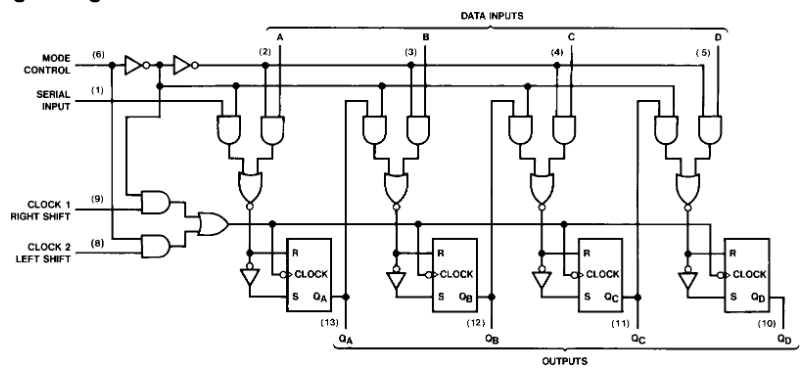
\includegraphics[scale=0.60]{7495_logic_diagram}‎
			\caption{اتصالات داخلی تراشه}
		\end{center}
	\end{figure} 

	\begin{figure}[h!]
	\begin{center}
		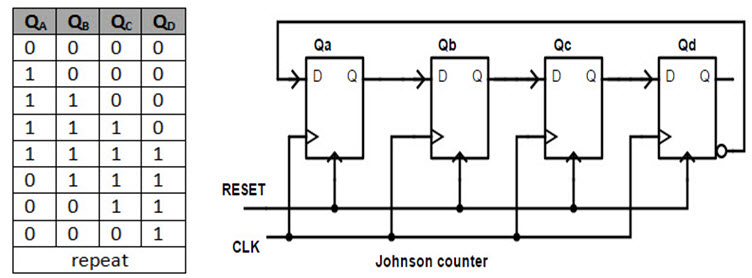
\includegraphics[scale=0.6]{johnson_ring_counter}‎
		\caption{شمارنده حلقه 4 بیتی}
	\end{center}
\end{figure} 

	\subsection*{مراحل آزمایش و مدارات}
	\begin{itemize}
		\item		
		برای قرار دادن مدار در حالت اولیه 1010 کافی است در مدار شکل 3 ، کلید PE فعال باشد و با دادن ورودی 1010 به پایه های A تا D ، شیفت رجیستر را به طور موازی پر کنیم.
		
		\item
		برای تغییر جهت شیفت رجیستر ، کافی است کلاک مربوط به شیفت راست را فعال کنیم و خروجی های هر $Q_{i}$ را به ورودی فلیپ فلاپ قبلی متصل کنیم.
		\item
		مطابق شکل مربوط به شمارنده جانسون ، کافی است با دادن ورودی
		 $ Q'_{D} $
		 به اولین فلیپ فلاپِ D ، یک شمارنده حلقه 4 بیتی تشکیل دهیم.
		 
		 \item
		 برای تبدیل شیفت رجیستر 4 بیتی به شیفت رجیستر دوطرفه ، کافی است هر خروجی
		 $ Q_{i} $
		 به ورودی قبلی خود یعنی $Q_{i-1}$ متصل باشد. پس باید یکی از ورودی های مالتی پلکسر ورودی هر فلیپ فلاپ باشد (توجه داریم ساختار انتخاب شده برای ورودی های فلیپ فلاپ های مدار ، معادل مالتی پلکسر های 2 به 1 هستند). حال با تغییر مقدار پایه کنترلی mode (پایه 6) میتوان همزمان کلاک مدار و جهت شیفت و ورودی های هر فلیپ فلاپ را تعیین کرد.
		 \item
		 برای طراحی مدار تشخیص دهنده الگو ها کافی است خروجی های شیفت رجیستر به طور موازی بررسی شوند و در نهایت با جمع مینترم های معادل ، یک گیت or خروجی را نشان دهد. با توجه به الگوهای خواسته شده کافی است جمع مینترم های 1 ، 2 ، 13 و 14 را به عنوان خروجی مدار تشخیص دهنده قرار دهیم. خروجی های فلیچ فلاپ ها و مینترم های گفته شده در شکل 3 مشخص اند.
		 
		 \begin{figure}[h!]
		 	\begin{center}
		 		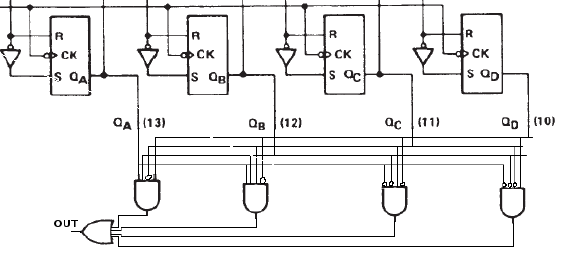
\includegraphics[scale=0.6]{pattern_finder}‎
		 		\caption{مدار تشخیص دهنده الگوها}
		 	\end{center}
		 \end{figure}
	 
	 \subsection*{نتایج مورد انتظار}
	 انتظار میرود با داشتن یک پالس ژنراتور ، دنباله اعمال ورودی پس از حداکثر تعداد 4 پالس کامل(با توجه به رفتار فلیپ فلاپ ها) در خروجی نمایش داده شوند.
		\begin{figure}[h!]
			\begin{center}
				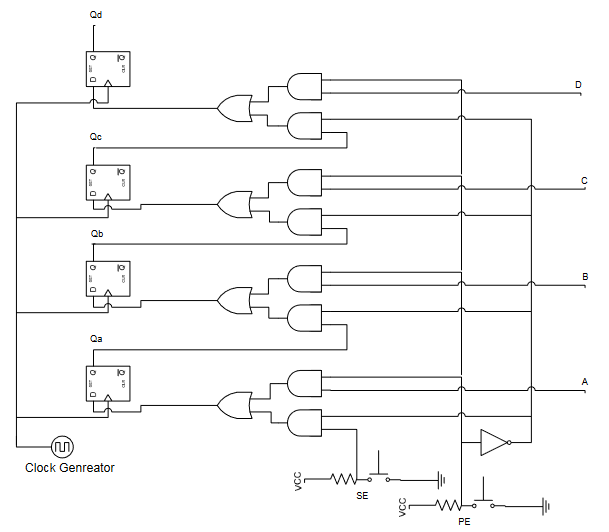
\includegraphics[scale=0.5]{suggested_circuit}‎
				\caption{مدار پیشنهادی برای شیفت رجیستر یک طرفه}
			\end{center}
		\end{figure} 
	
		\begin{figure}[h!]
			\begin{center}
				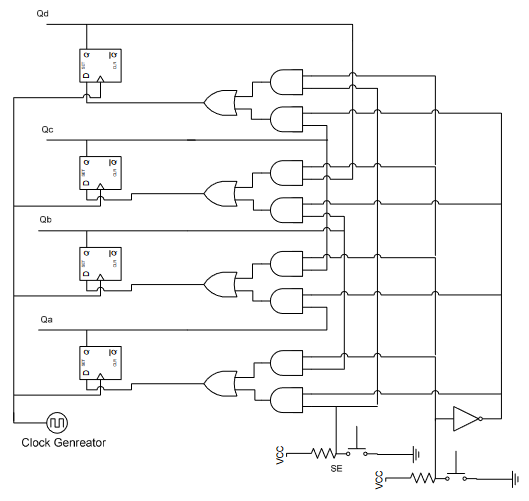
\includegraphics[scale=0.5]{suggested_circuit_2}‎
				\caption{مدار پیشنهادی برای شیفت رجیستر دو طرفه}
			\end{center}
		\end{figure} 
	\end{itemize}

	
	\begin{figure}[h!]
		\begin{center}
			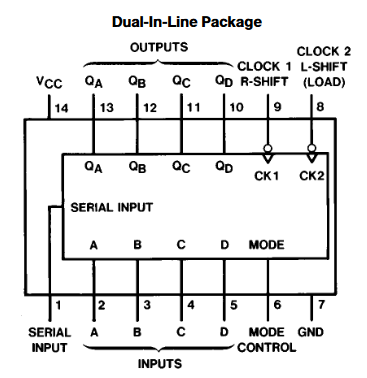
\includegraphics[scale=0.75]{7495_connection_diagram}‎
			\caption{تراشه 7495}
		\end{center}
	\end{figure} 

	\begin{figure}[h!]
		\begin{center}
			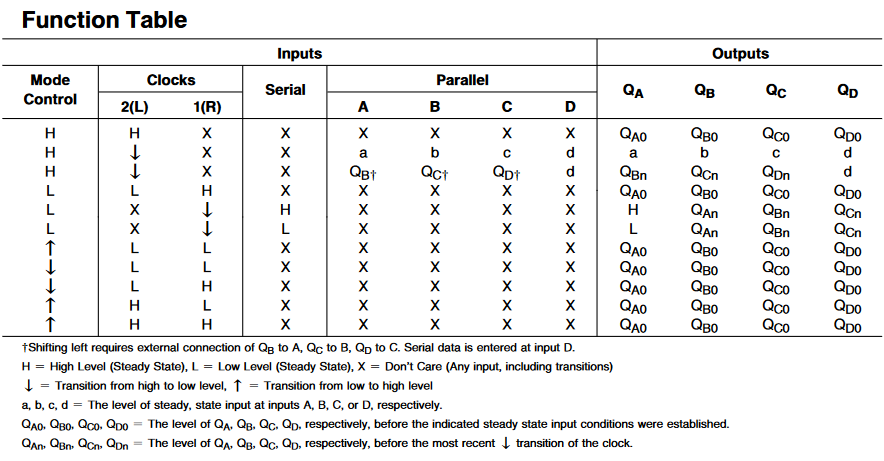
\includegraphics[scale=0.6]{7495_function_table}‎
			\caption{ جدول عملکردی تراشه 7495}
		\end{center}
	\end{figure} 

\end{document}









